In this section, basic approaches how to focus a laser beam in experiments are discussed. Before providing a brief overview of currently used methods, it is necessary to introduce several most fundamental parameters that describe any optical system. First, one defines a numerical aperture of an optical system $ N\!A $, which is a dimensionless number characterizing the range of angles over which the system can accept or emit light. Second characteristic of any optical system is a focal length $ f $ describing a distance between the center of the aperture and the point in space over which collimated light rays are brought to a focus. Finally, one defines a f-number $ f/\# $ as a ratio of the focal length $ f $ to the size of the aperture $ D $. The f-number $ f/\# $ is dimensionless and stands for a quantitative measure of a speed of the optical system.

In experiments, tight-focusing of laser beams is usually achieved by means of an optical system, such as a lens or a curved mirror. However, when dealing with a short pulses, lenses are not preferred because they may affect the beam by frequency-dependent effects, such as chromatic aberration and other nonlinear optical distortions. On the other hand, reflective optics are generally able to produce a diffraction limited image without chromatic effects.

An off-axis parabolic (OAP) mirror is a frequently used tool to focus an incoming collimated beam. OAP is made by cutting out a small section from a full parabolic mirror and thus it allows to deviate the beam path off the optical axis. Therefore, the parts of incoming collimated beam do not overlap as in the case of a complete parabolic mirror and the focal spot is at more accessible location. Obviously, OAP is able to work reversibly, so it can take the light coming from a point source and produce a collimated beam. These physical properties make OAP a valuable tool for many different optical purposes.

Lens, off-axis parabola mirror - conventional solid state optic
ellipsoid plasma mirrors, plasma lens



\floatsetup[figure]{style=plain, subcapbesideposition=top}
\begin{figure}[h!]
	\centering
	\sidesubfloat[]{{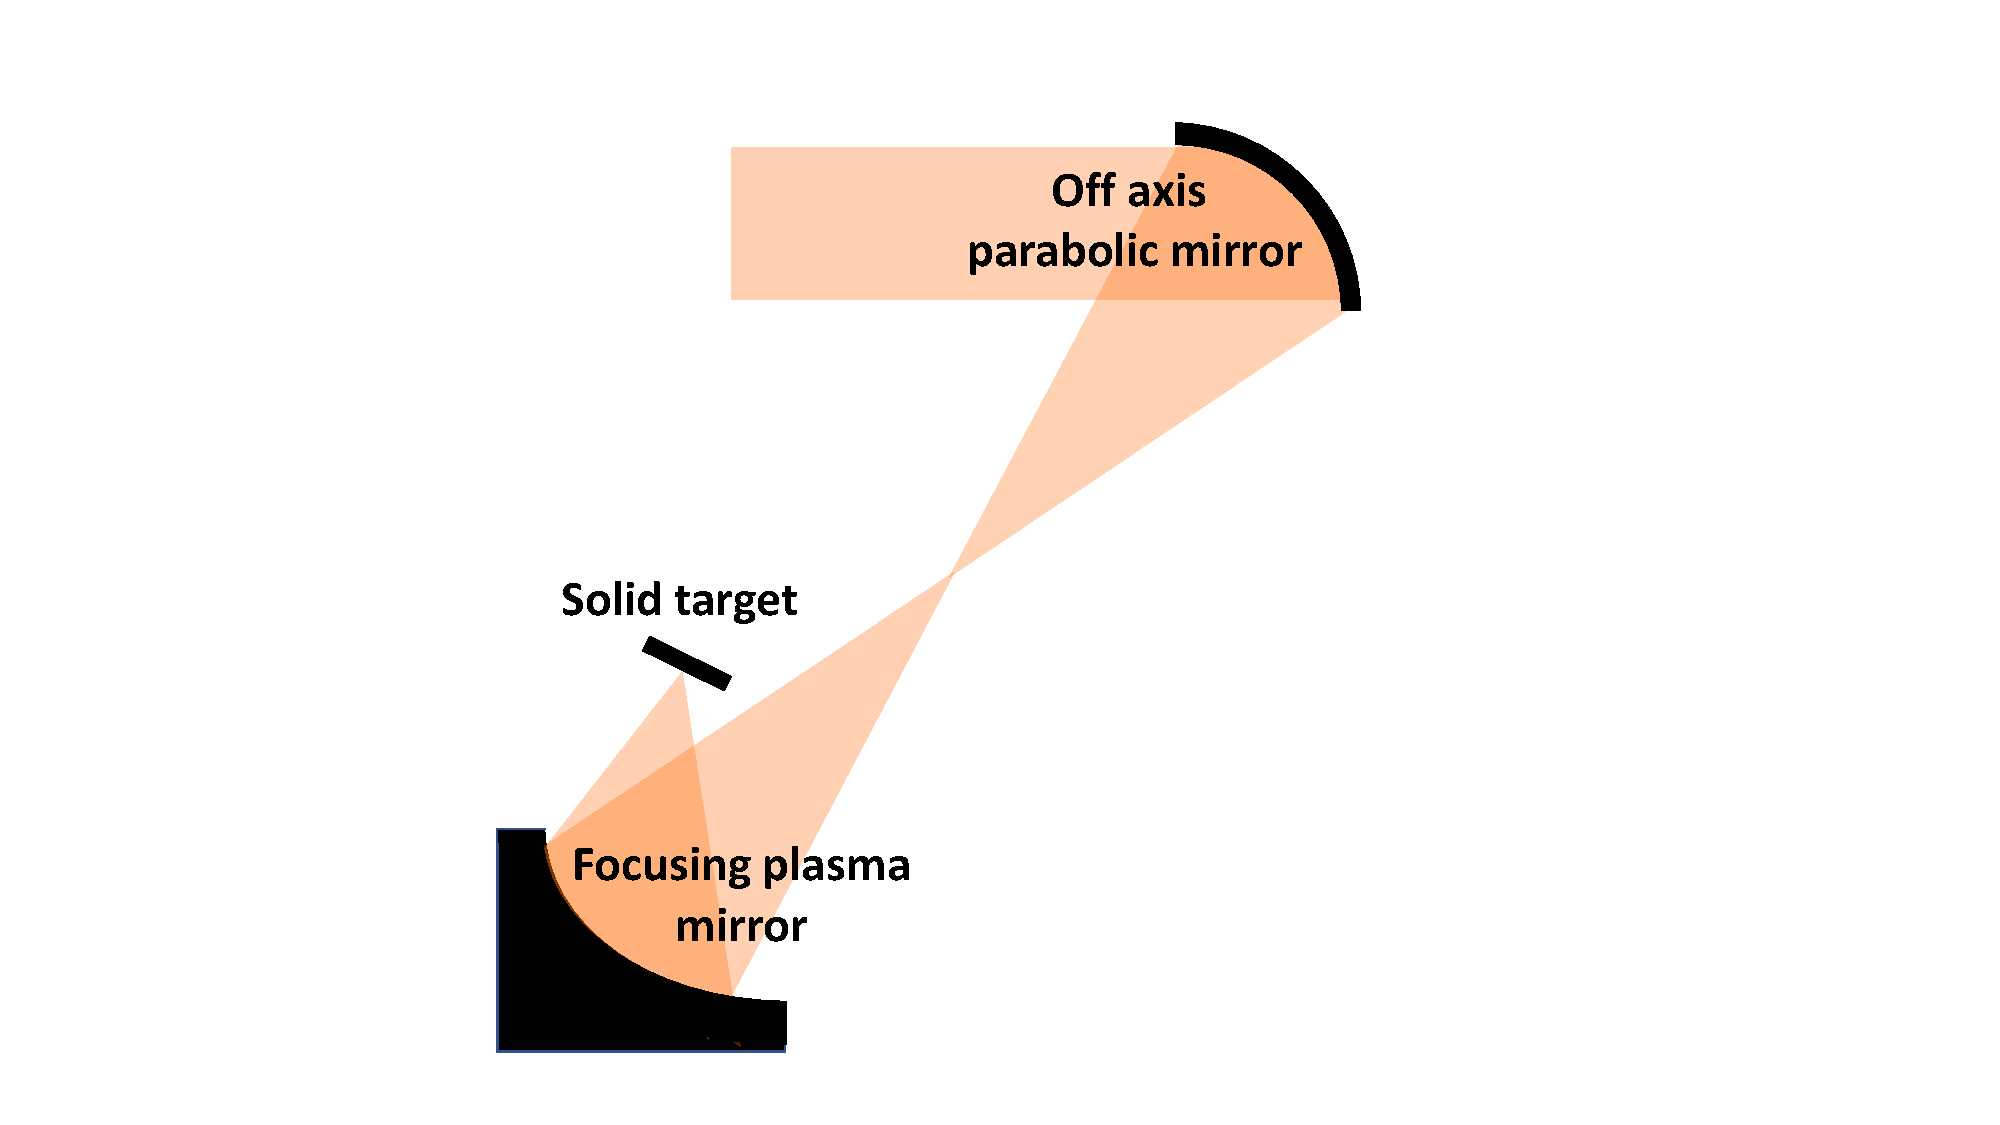
\includegraphics[width=0.35\linewidth]{./img/exp/diagram.pdf}}}
	\hspace{5mm}
	\sidesubfloat[]{{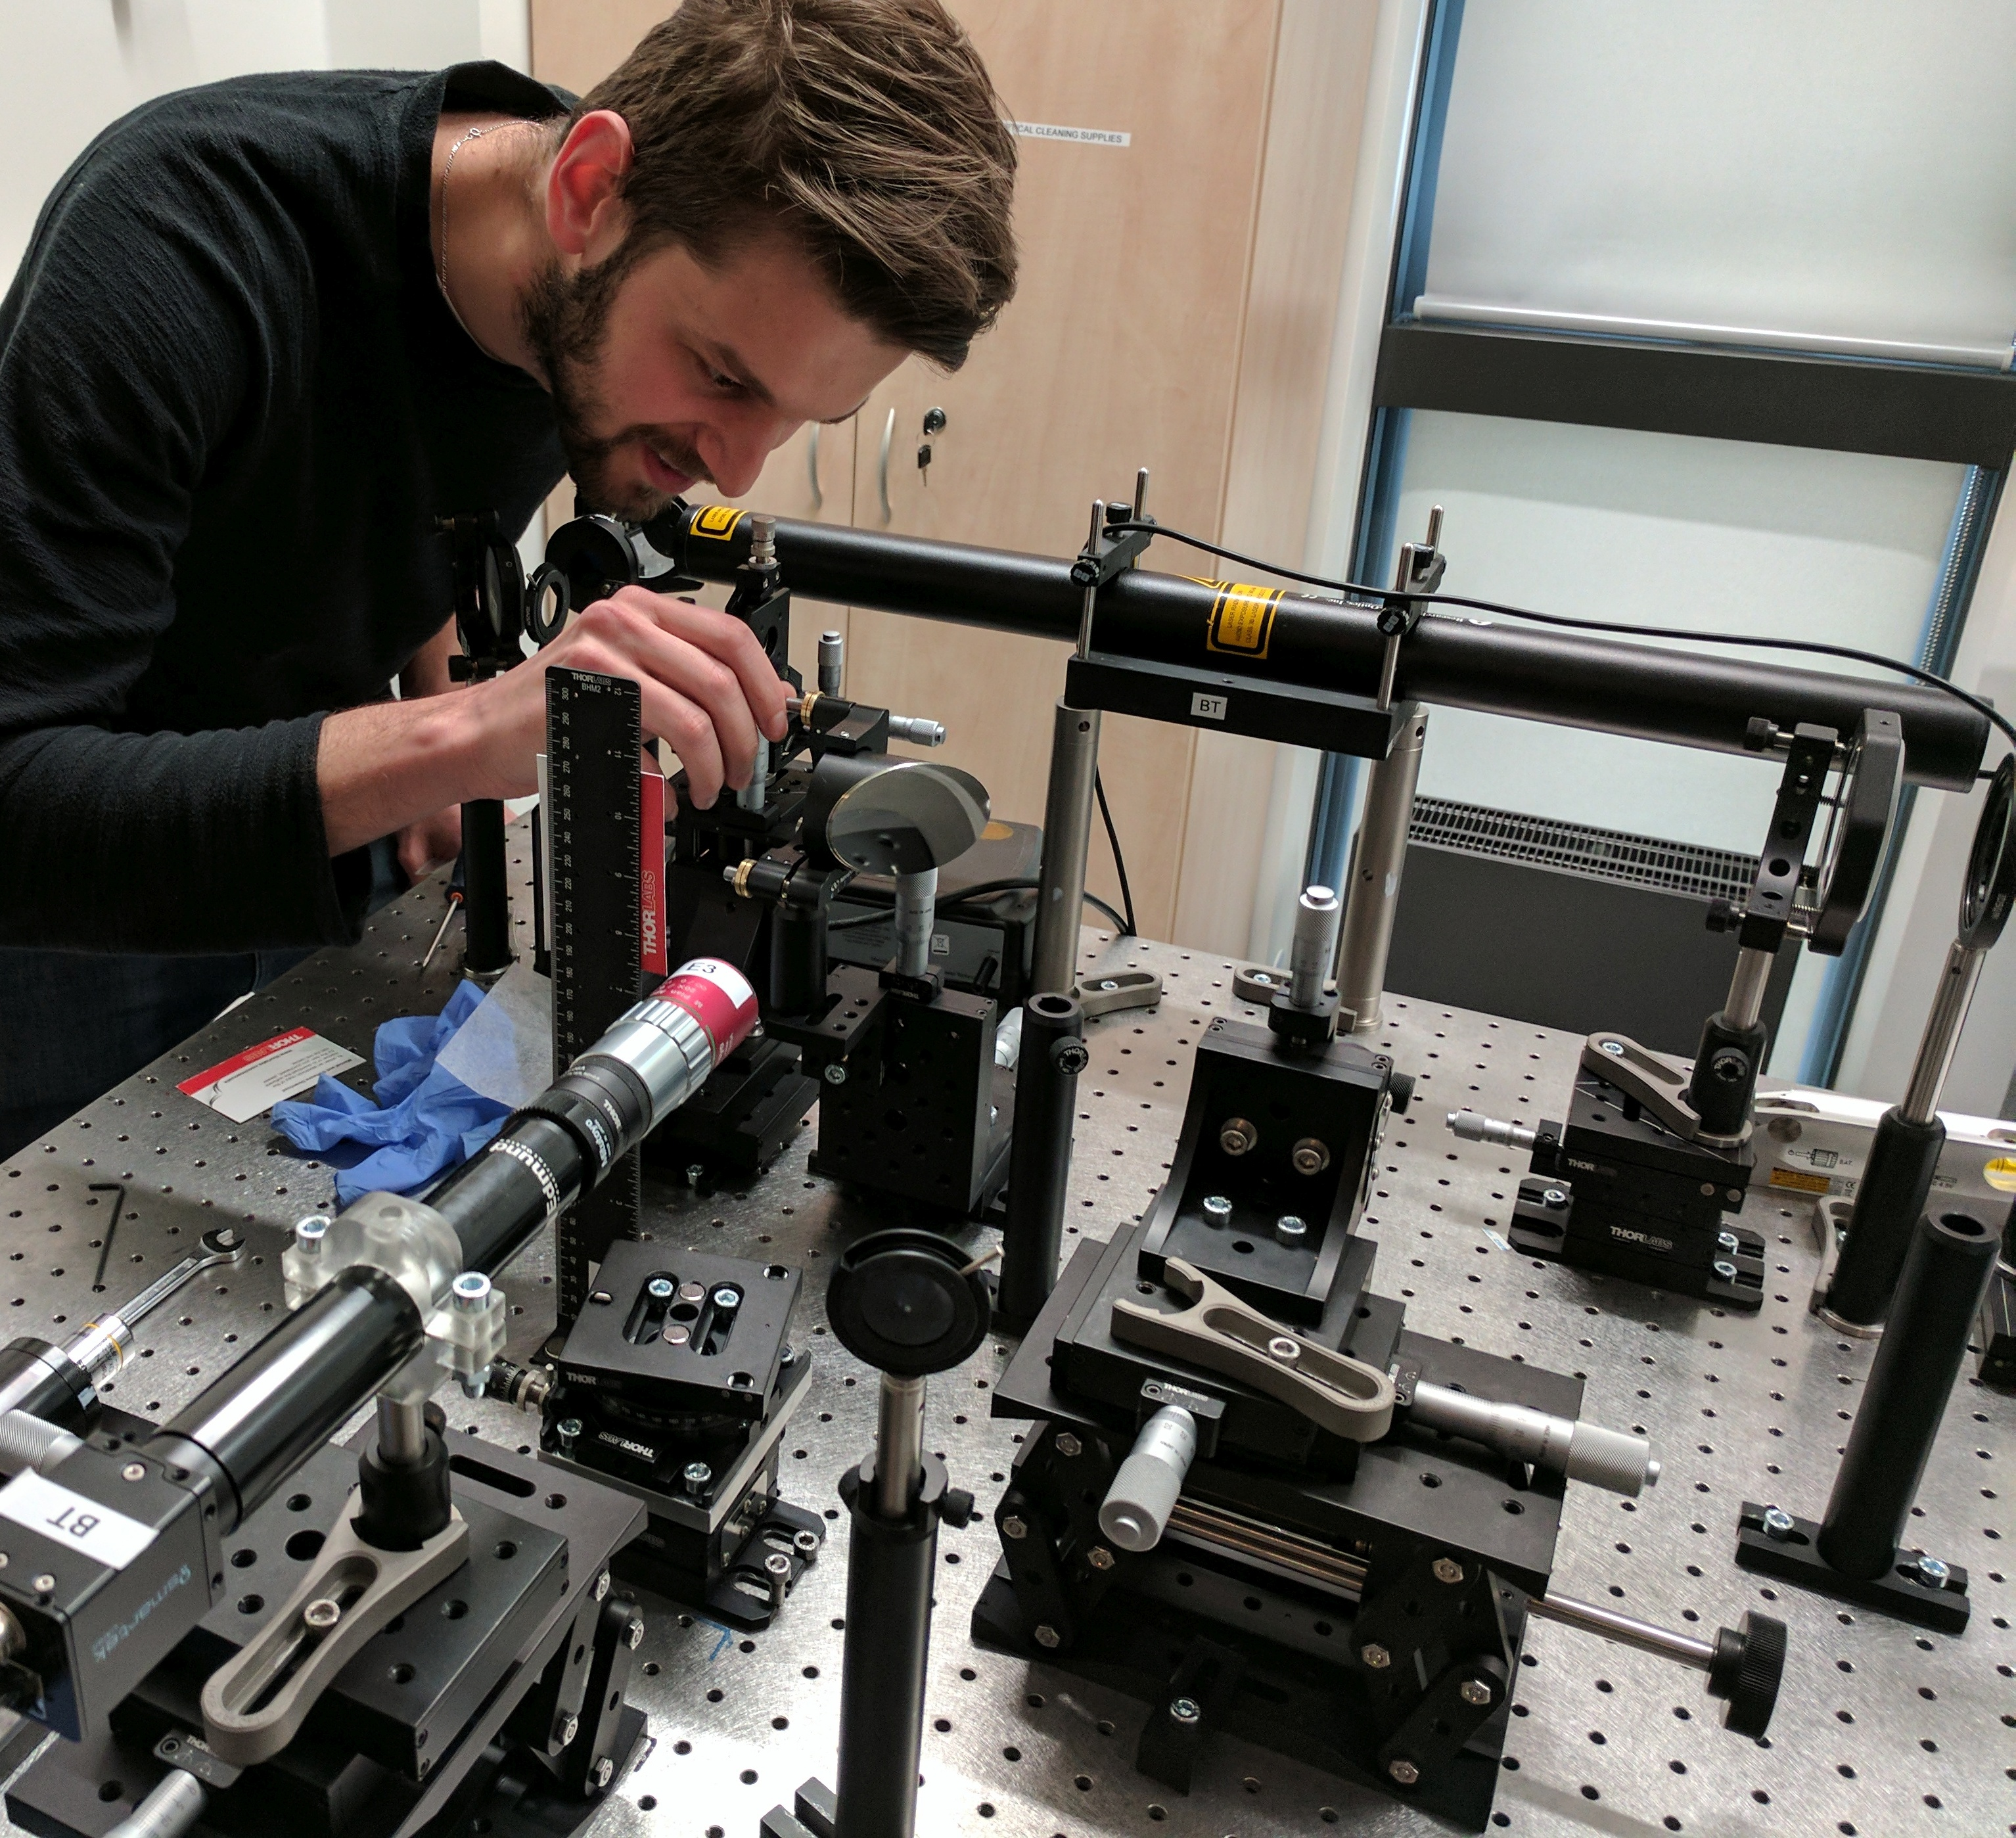
\includegraphics[width=0.4\linewidth]{./img/exp/photo2.jpg}}}
	\caption{\textbf{(a)} Schematic diagram showing the operation of the focusing plasma mirror where the incoming laser beam is focused by a conventional off-axis parabolic mirror. The plasma mirror focuses the beam onto a target surface. \textbf{(b)} Photo capturing a very long and frustrating process of aligning an off-axis parabolic mirror.}
	\label{}
\end{figure}